\subsection{Example 1}
Lets say one needs to get the title of all the patents that had been invented in Texas between the period January 2005 and February 2005. To do this, perform the following steps (screenshots shown after the steps): 

\begin{enumerate}
\item Select the checkbox besides “Title of Patent” in primary information.

\item In the filters section, under Primary information, set From as 2005-1-1 and To as 2005-2-1. Also, type ‘TX’ in inventor’s state textbox. 

\item Finally, type in your email address on the bottom of the page, choose the filetype, and click on “Submit”.
\end{enumerate}

This form is translated into the SQL query:

SELECT patent.title FROM patent, rawinventor, rawlocation WHERE (patent.date BETWEEN ‘2005-1-1’ AND ‘2005-2-1’) AND (patent.id = rawinventor.patent\_id) AND ((rawlocation.state LIKE ‘\%TX\%’) AND rawlocation.id = rawinventor.rawlocation\_id);

\begin{figure*}
\center
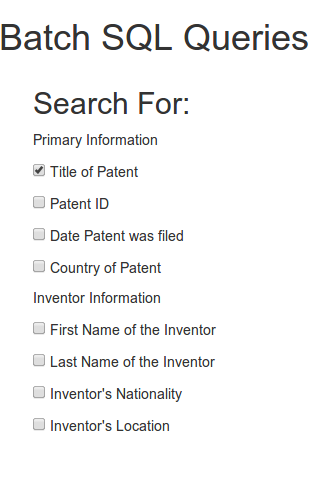
\includegraphics[width=.8\textwidth]{figs/ex1s1}
\caption{Example 1: Step 1}
\label{fig:Step 1}
\end{figure*}

\begin{figure*}
\center
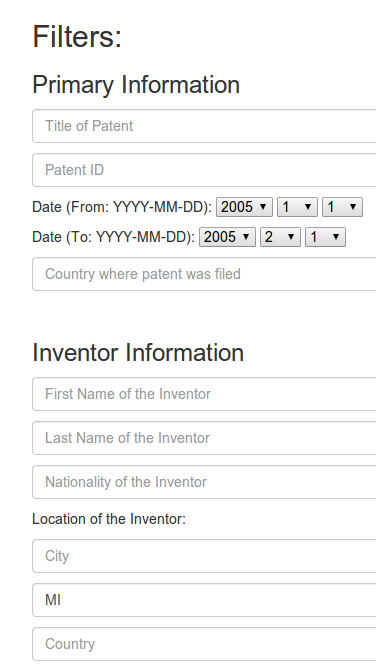
\includegraphics[width=.8\textwidth]{figs/ex1s2}
\caption{Example 1: Step 2}
\label{fig:Step 2}
\end{figure*}

\begin{figure*}
\center
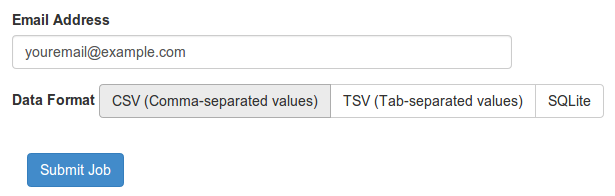
\includegraphics[width=.8\textwidth]{figs/ex1s3}
\caption{Example 1: Step 3}
\label{fig:Step 3}
\end{figure*}


\subsection{Example 2}
For the second example, lets say one needs to get the names (first and last) of the lawyers that filed for a patent in Michigan between January 2005 and February 2005. In addition, say they want the inventors and assignees to also be in Michigan$^{[5]}$.

\begin{enumerate}

\item Select First Name of Lawyer and Last Name of Lawyer under Lawyer Information.

\item In the filters section, make sure to fill in dates as before, and this time, fill in the textbox for Inventors State with ‘MI’ and same for the Assignee’s State textbox.

\item Finally, just as before, fill in your email, choose your filetype, and click on “Submit”.

\end{enumerate}

This form is translated into the SQL query:

SELECT rawlawyer.name\_first, rawlawyer.name\_last FROM patent, rawlocation, rawinventor, rawassignee, rawlawyer WHERE (patent.date BETWEEN ‘2005-1-1’ AND ‘2005-2-1’) AND (patent.id = rawinventor.patent\_id) AND (rawassignee.patent\_id = rawinventor.patent\_id) AND (rawlawyer.patent\_id = rawinventor.patent\_id) AND ((rawlocation.state LIKE ‘\%MI\%’) AND rawlocation.id = rawinventor.rawlocation\_id) AND ((rawlocation.state LIKE ‘\%MI\%’) AND rawlocation.id = rawassignee.rawlocation\_id);

\begin{figure*}
\center
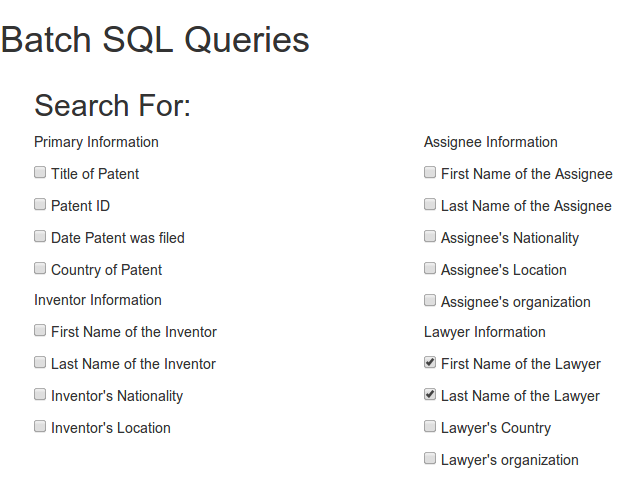
\includegraphics[width=.8\textwidth]{figs/ex2s1}
\caption{Example 2: Step 1}
\label{fig:Step 1}
\end{figure*}

\begin{figure*}
\center
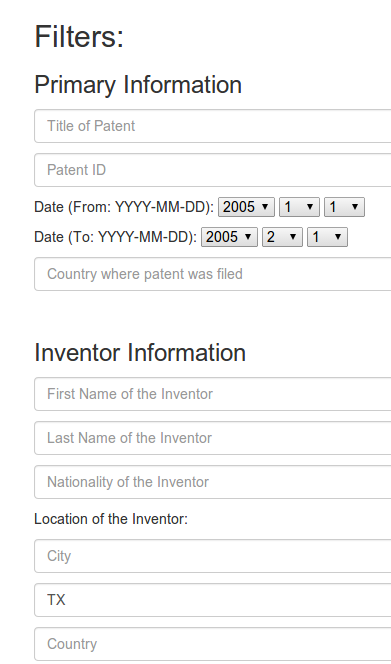
\includegraphics[width=.8\textwidth]{figs/ex2s2-1}
\caption{Example 2: Step 2-1}
\label{fig:Step 2}
\end{figure*}

\begin{figure*}
\center
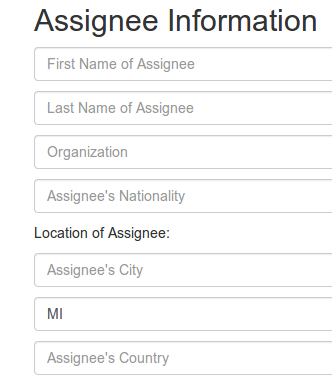
\includegraphics[width=.8\textwidth]{figs/ex2s2-2}
\caption{Example 2: Step 2-2}
\label{fig:Step 3}
\end{figure*}

